% Created 2021-01-24 Sun 22:49
% Intended LaTeX compiler: pdflatex
\documentclass[11pt]{article}
\usepackage[utf8]{inputenc}
\usepackage[T1]{fontenc}
\usepackage{graphicx}
\usepackage{grffile}
\usepackage{longtable}
\usepackage{wrapfig}
\usepackage{rotating}
\usepackage[normalem]{ulem}
\usepackage{amsmath}
\usepackage{textcomp}
\usepackage{amssymb}
\usepackage{capt-of}
\usepackage{hyperref}
\usepackage{minted}
\hypersetup{colorlinks=true, linkcolor=black, filecolor=red, urlcolor=blue}
\usepackage[turkish]{babel}
\author{Eren Hatırnaz}
\date{5 Nisan 2020}
\title{Yazılım Gündemi - 2020/13\\\medskip
\large 30 Mart - 5 Nisan 2020}
\hypersetup{
 pdfauthor={Eren Hatırnaz},
 pdftitle={Yazılım Gündemi - 2020/13},
 pdfkeywords={},
 pdfsubject={},
 pdfcreator={Emacs 27.1 (Org mode 9.3)},
 pdflang={Turkish}}
\begin{document}

\maketitle
\tableofcontents \clearpage\shorthandoff{=}

\begin{center}
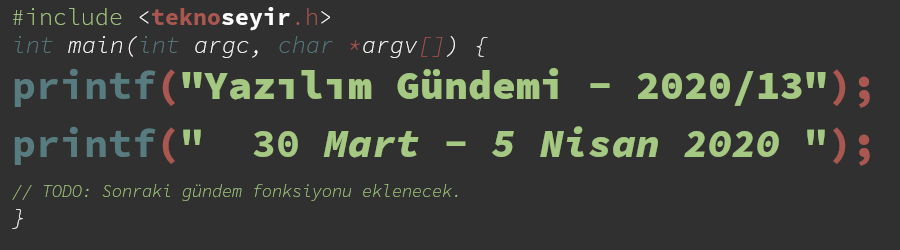
\includegraphics[width=.9\linewidth]{gorseller/yazilim-gundemi-banner.png}
\end{center}

\begin{center}
\href{../12/yazilim-gundemi-2020-12.pdf}{< Önceki Gündem} | \textbf{30 Mart - 5 Nisan 2020} | \href{../14/yazilim-gundemi-2020-14.pdf}{Sonraki Gündem >}

\href{https://teknoseyir.com/blog/yazilim-gundemi-2020-13}{TeknoSeyir'de Oku}
\end{center}

\section{Chromium tabanlı tarayıcılarda \href{https://blog.chromium.org/2020/03/updates-to-form-controls-and-focus.html}{form elemanlarının varsayılan görünümü değişiyor}}
\label{sec:org36bd09f}
Microsoft'un yeni Edge tarayıcısının ve Google'ın Chrome tarayıcısının da
kullandığı Chromium açık kaynaklı tarayıcısının bu hafta blogunda yayınlanan
yazı ile artık form kontrollerinin işletim sistemi değişmeksizin aynı
görüneceği duyuruldu. Sorunun ne olduğunu anlamak için web geliştirme yapmış
kişilerin mutlaka bir dönem kullandığı belki hala daha kullanıyor olduğu
"reset.css" dosyasını hatırlatmak isterim. Hatırlamayan ya da bilmeyenler için
bu dosya işletim sistemi ve tarayıcılardan kaynaklanan stil farklılıklarını
temizleyen bir css dosyası. Sayfaya önce bu css dosyası eklenir, daha sonra
kendi özel css dosyalarımız eklenirdi ki sayfamız tüm tarayıcılarda ve işletim
sistemlerinde aynı gözüksün. Modern web dünyasında eskisi kadar ihtiyaç
duymasak da Google Chromium ve Microsoft Edge takımları bunu dert edinmişler.

\begin{figure}[htbp]
\centering
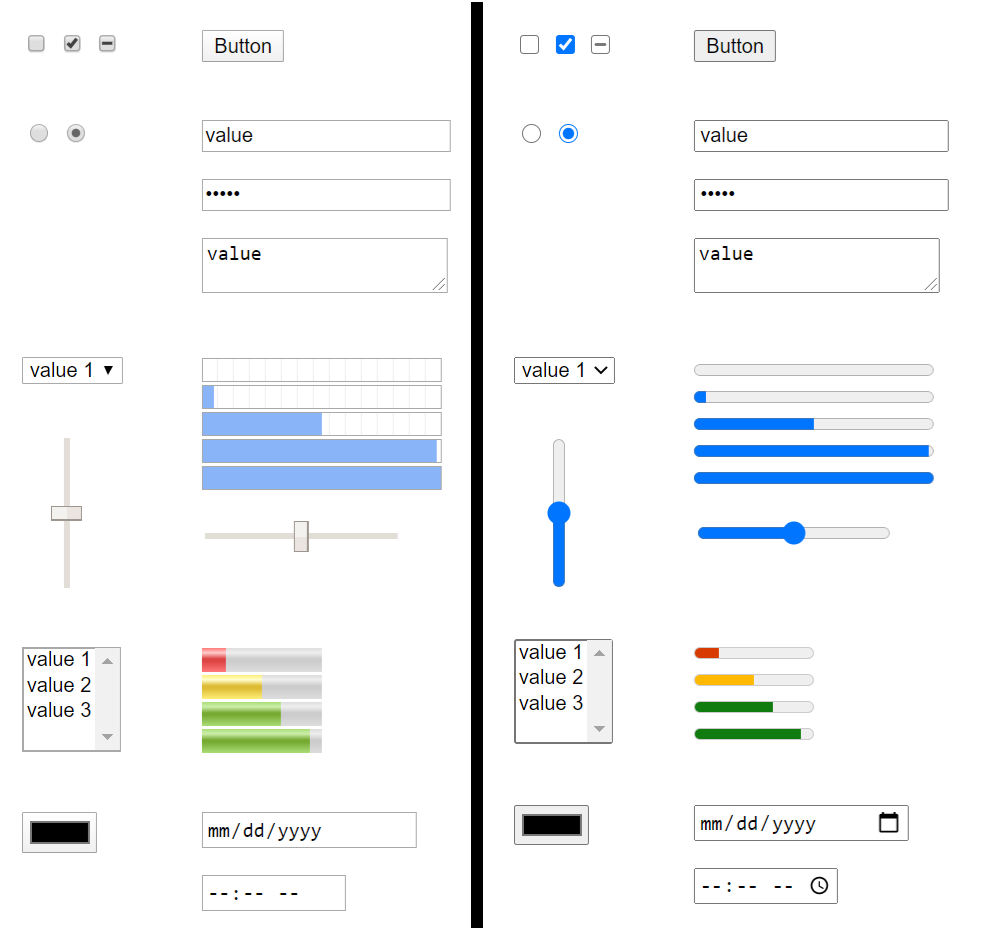
\includegraphics[width=.9\linewidth]{gorseller/chromium-form-eski-yeni.png}
\caption[\textbf{(SOL):} \textbf{(SAĞ):}]{\textbf{(SOL):} Chrome 80 ve önceki sürümlerdeki stillendirme. \textbf{(SAĞ):} Yeniden tasarlanan form elemanları.}
\end{figure}

Google'ın Chromium takımı ve Microsoft'un Edge takımının birlikte çalışması
sonucu oluşmuş bu yeni form elemanları tasarımları Edge tarayıcısının son
sürümünde kullanılmış fakat Chrome'un 81 numaralı sürümünde deneysel olarak
kullanıma açılacakmış. Chrome 81'de bu tasarıma geçmek için:
chrome://flags/\#form-controls-refresh özelliğini aktifleştirmek yeterli olacak
deniyor.

\url{gorseller/chromium-focus-ring.gif}

Aynı zamanda tarayıcıdaki bağlantı ve objeler üzerinde gezinmek için
kullanabildiğimiz TAB tuşuyla birlikte ortaya çıkan "focus halkası" (focus
ring) de yenilenmiş. Daha görünür olması için siyah renk ve beyaz çerçeve
tercih edilmiş. Yine de bazı durumlarda görünmez olabileceği söylenmiş.

Yapılan diğer değişiklik ve yeniden tasarımlar için konu başlığına eklediğim
bağlantıya tıklayabilirsiniz.

Sizce yeni tasarımlar nasıl oldu? Böyle bir değişikliğe gerek var mıydı?
Yorumlar bölümünde konuşalım.
\section{GitLab, 18 tane özelliğini \href{https://about.gitlab.com/blog/2020/03/30/new-features-to-core/}{açık kaynak yapmaya hazırlanıyor}}
\label{sec:org28e1f2a}
Popüler uzak git sunucularından biri olan GitLab, bu hafta içerisinde
yayınladıkları bir blog yazısı ile birlikte normalde ücretli sürümde olan 18
adet özelliği açık kaynak olan sürüme getireceklerini duyurdular. Fakat ilginç
bir yöntemle. Özellikler GitLab'in şu 7 parçasının içerisinden alınacakmış:
\href{https://about.gitlab.com/features/\#plan}{Plan}, \href{https://about.gitlab.com/features/\#create}{Create}, \href{https://about.gitlab.com/features/\#verify}{Verify}, \href{https://about.gitlab.com/features/\#release}{Release}, \href{https://about.gitlab.com/features/\#configure}{Configure}, \href{https://about.gitlab.com/features/\#defend}{Defend}.

\begin{figure}[htbp]
\centering
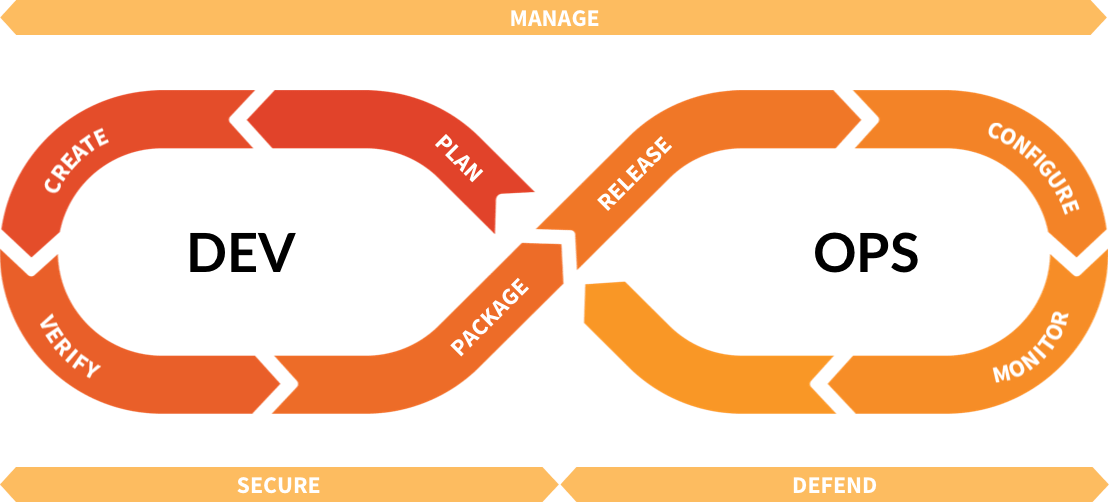
\includegraphics[width=.9\linewidth]{gorseller/gitlab-devops-plan.png}
\caption{Yani Monitor hariç DevOps sürecinin diğer tüm kısımlardan bir şeyler açık kaynak olacak}
\end{figure}

İlginç bir yöntem dedim çünkü bu özellikleri açık kaynak yapmak için
topluluktan yardım istiyorlar. \href{https://gitlab.com/gitlab-org/gitlab/-/issues/212330}{Issue Export}'dan, \href{https://gitlab.com/gitlab-org/gitlab/-/issues/211685}{Web IDE'si için Web
Terminal}'a kadar birçok konuda "gelin bunları birlikte açık kaynak yapalım"
diyorlar. Konu başlığına eklediğim blog yazısında açık kaynak yapmak
istedikleri her özellik için açılan issue sayfalarının linklerini vermişler.
İlgili issue sayfalarında yapılacaklarla ilgili bilgiler vermişler. Böylece
insanlar da o konularla ilgili yardım edebiliyor.

Sonuçta GitLab'ın ücretli sürümünün kaynak kodlarına erişimi olan onlar ve
doğal olarak oradan kendileri de açık kaynak hale getirebilirler ilgili
parçaları (içerdeki kod yapısı hakkında bilgim yok tabii). Topluluktan yardım
istemeleri bana biraz tuhaf geldi. Neyse yine de bizim işimize yarayacak
şeyler olduğu için fazla kurcalamayayım :).
\section{Eclipse, VSCode alternatifi IDE'sini \href{https://www.eclipse.org/org/press-release/20200331-theia.php}{açık kaynak olarak duyurdu}: \href{https://theia-ide.org/\#features}{Eclipse Theia}}
\label{sec:org2733a55}
Daha çok Java için IDE'si olmakta tanınan ama başka çözümleri de bulunan
Eclipse Foundation, bu hafta içerisinde yeni hem bulutta hem de masaüstünde
çalışabilen IDE'sini açık kaynak olarak tanıttı.

Proje aslında 2016 yılında \href{https://www.ericsson.com/en}{Ericsson} ve \href{https://www.typefox.io/}{TypeFox} firmaları tarafından
başlatılmış fakat zamanla Eclipse Foundation gibi birçok firmanın katkılarıyla
bu hale gelmiş. Proje şu an Eclipse Foundation altındaki \href{https://ecdtools.eclipse.org/}{Eclipse Cloud
Development Tools Working Group} (ECD WG) tarafından devam ettiriliyor. Aynı
zamanda açık kaynakta olduğu için topluluğun katkılarına açık. Aynı zamanda
Google Cloud, RedHat, Arduino, IBM gibi firmalar da projeye katkı yapmışlar.

\begin{center}
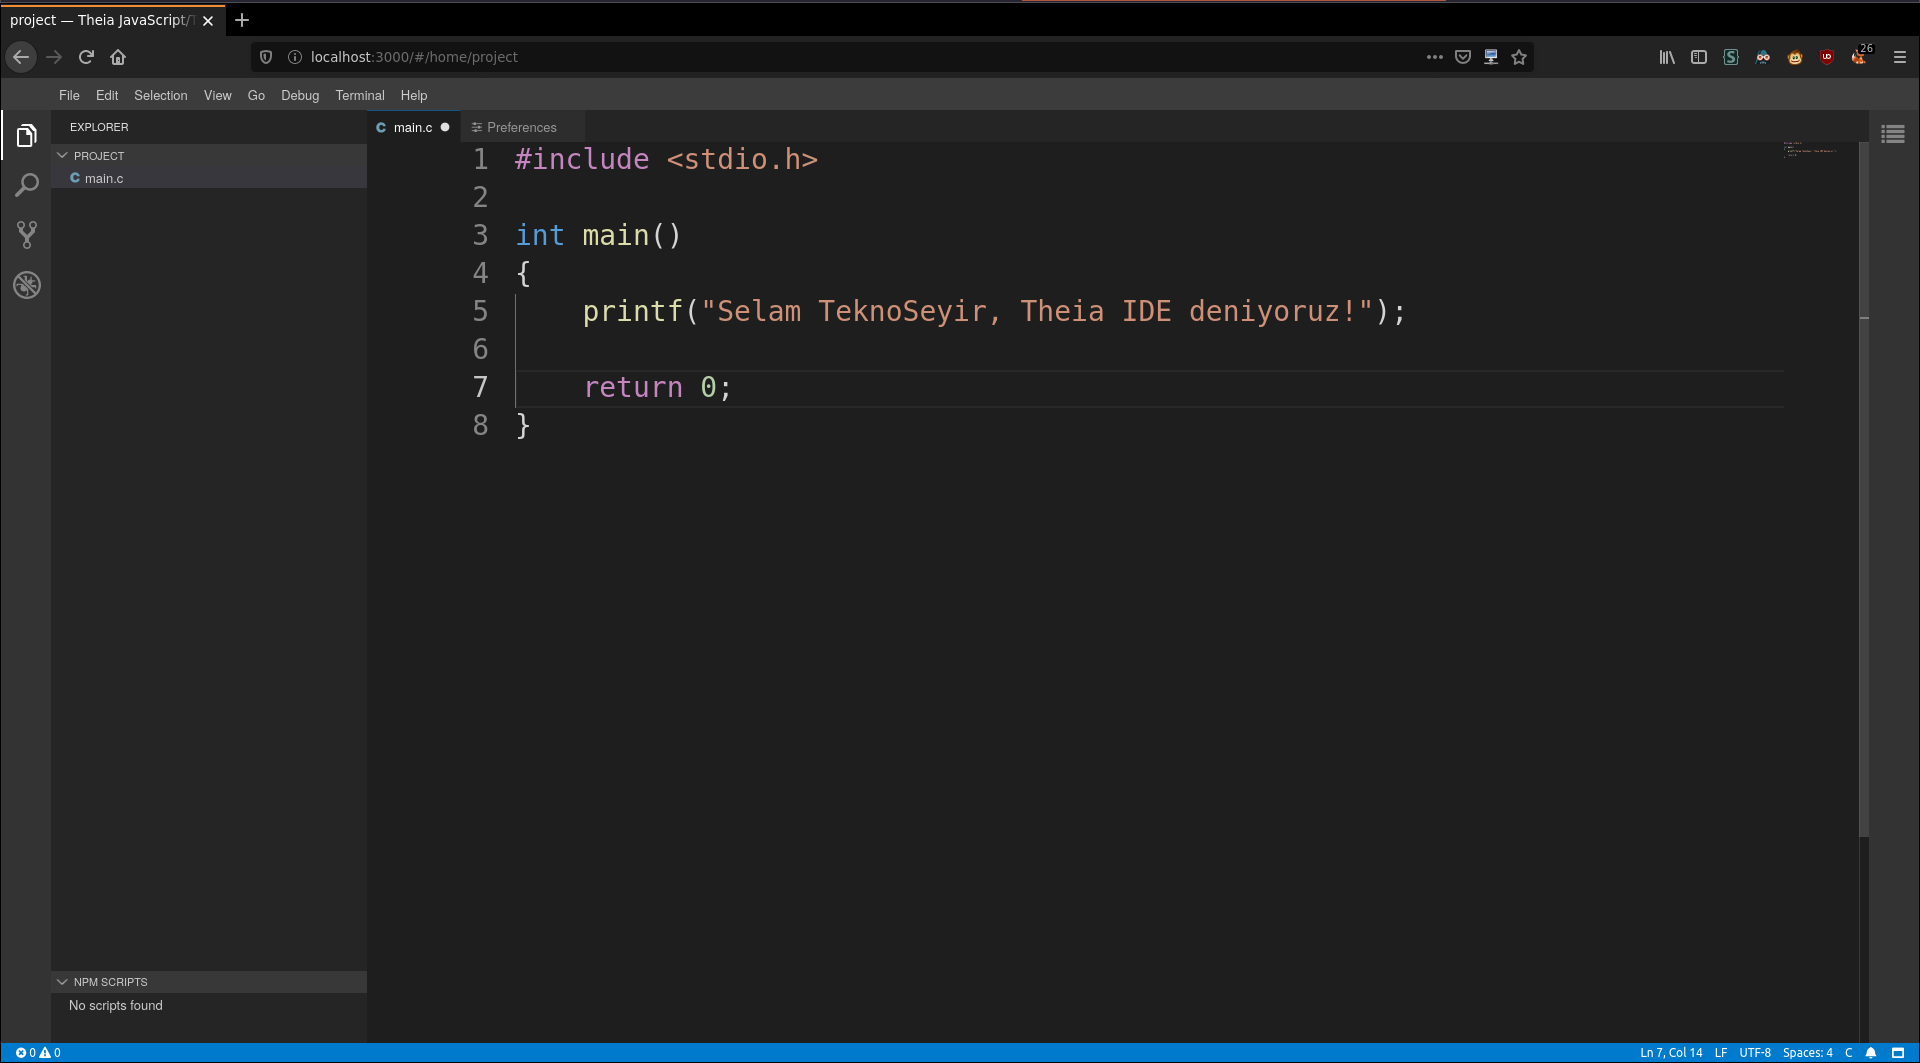
\includegraphics[width=.9\linewidth]{gorseller/eclipse-theia-demo.png}
\end{center}

Eclipse'in duyuru yazısında VSCode eklentilerini de bu IDE'de
çalıştırabiliyorsunuz diyor fakat ben denemedim. Aynı yazıda Eclipse Theia ile
VS Code arasındaki farklar olarak şu üç madde sıralanmış:

\begin{itemize}
\item Theia'nın mimarisi daha modüler ve özelleştirmelere daha uygun.
\item Theia hem masaüstünde hem de bulutta çalışabiliyor.
\item Theia topluluk-destekli ve Eclipse Foundation'ın bağımsız yönetimi
tarafından geliştiriliyor.
\end{itemize}

Son maddeyi ben de tam anlamadım. VS Code'da zaten açık kaynak olduğu için
topluluk katkı yapabiliyor ve Microsoft sürümlerini yayınlıyor. Büyük ihtimal
yanlış anlamış ve çevirmiş olabilirim. Eğer yanlış anlamışsan, yorumlar
bölümünde beni düzeltmekten kendinizi geri koymayın.

IDE'nin masaüstü uygulaması \href{https://www.electronjs.org/}{Electron} tabanlı ve uzaktaki sunucu ile \href{https://www.jsonrpc.org/specification}{JSON-RPC}
mesajlarını HTTP ya da WebSocket üzerinden ileterek çalışıyor. Ben docker
kullanarak kendi bilgisayarıma kurdum ve biraz kurcaladım. Eğer siz de denemek
isterseniz bilgisayarınıza Docker kurduktan sonra aşağıdaki komutu açmak
istediğiniz proje dizinindeyken çalıştırabilirsiniz (yalnız dosya kaydetme
kısmında izinlerle ilgili bir hata veriyor, pek uğraşamadım çözmek için):

\begin{minted}[breaklines=true,breakanywhere=true]{bash}
docker run --rm -it -p 3000:3000 -v "$(pwd):/home/project:cached" theiaide/theia
\end{minted}

Bu yazılım gündemi yazılarını yazmaya başladığımdan beri fark ettim ki son bir
yıldır herkes geliştiricilere bir uzaktan geliştirme çözümü üretmeye
çalışıyor. Önümüzdeki birkaç senede popülerliği daha da artacaktır diye
umuyorum "Cloud Development" (ya da ileride ne isim verirlerse) olayının. Siz
bu konuda ne düşünüyorsunuz? Bu tarz çözümleri kullanır mıydınız ya da
kullanıyor musunuz? yoksa "yok arkadaş ben o kadar yenilikçi değilim eski tip
masaüstü uygulaması IDE ya da metin editörümle iyiyim" diyenlerden misiniz?
yorumlar bölümünde konuşalım.
\section{Covid-19 Pandemisi, NodeJS sürüm \href{https://nodejs.org/en/blog/announcements/adjusted-release-schedule-covid/}{yayınlama takvimini de etkiledi}}
\label{sec:orgb7eff4f}
Tüm dünya olarak içinde bulunduğumuz süreçten elbette yazılım sektörü de
payını almaya devam ediyor. Her ne kadar uzaktan çalışmaya en uygun
mesleklerden biri bizimki olsa da, pratikte bazı şeyler düşünüldüğü gibi
olmuyor. NodeJS takımı da olası sorunların önüne geçmek amacıyla bu hafta
sürüm yayınlama takvimini güncelledi. Buna göre:

\begin{itemize}
\item \texttt{v10.x} ve \texttt{v12.x} dallarındaki bir sonraki sürüm 7 Nisan tarihinde çıkacak.
\item \texttt{v12.x} dalındaki minor sürüm numaralarının yanın tarihleri ertelendi:
\begin{itemize}
\item \texttt{v12.17.0}: 26 Mayıs 2020
\item \texttt{v12.18.0}: 25 Ağustos 2020
\end{itemize}
\item \texttt{v13.x} dalında, End of Life (hayatının sonu) tarihi olan Haziran 2020'ye
kadar yeni bir sürüm yok.
\item \texttt{v14.x} dalının ilk sürümü ise planlandığı gibi 21 Nisan 2020 tarihinde
yayınlanacakmış.
\end{itemize}

Tarihlerle ilgili daha detaylı bilgiler için konu başlığına eklediğim
bağlantıya tıklayabilirsiniz.
\section{PHP 8 sürümünün \href{https://wiki.php.net/todo/php80}{yayın takvimi belli oldu}}
\label{sec:orgb93c4b4}
Aşağıdaki sürümlerin hepsi 2020 yılı içerisinde çıkacak.

\begin{center}
\begin{tabular}{ll}
Sürüm & Yayınlanma Tarihi\\
\hline
18 Haziran & Alpha 1\\
2 Temmuz & Alpha 2\\
16 Temmuz & Alpha 3\\
27 Temmuz & Feature freeze\\
20 Temmuz & Beta 1\\
13 Ağustos & Beta 2\\
27 Ağustos & Beta 3\\
10 Eylül & Relase Candidate 1\\
24 Eylül & Relase Candidate 2\\
8 Ekim & Release Candidate 3\\
22 Ekim & Release Candidate 4\\
5 Kasım & Release Candidate 5\\
19 Kasım & Release Candidate 6\\
3 Aralık & Genel Erişilebilirlik (Final)\\
\end{tabular}
\end{center}
\section{Safari 13.1 ile \href{https://webkit.org/blog/10247/new-webkit-features-in-safari-13-1/}{gelen yenilikler}}
\label{sec:org5039ca2}
Geçtiğimiz haftaki yazılım gündemi yazısında (bkz: \href{../12/yazilim-gundemi-2020-12.pdf}{Yazılım Gündemi - 2020/12})
Safari 13.1 ile birlikte tüm üçüncü parti çerezlerin engellenmeye başlandığını
söylemiştim. Bu hafta ise Safari 13.1 ile birlikte gelen ve biz
geliştiricileri ilgilendiren diğer birkaç özelliğe birlikte göz atalım.

\subsection{JavaScript iyileştirlemeleri}
\label{sec:orgb12029c}
Safari tarayıcısının bu sürümüyle birlikte artık \texttt{replaceAll()} fonksiyonu
desteklenmeye başlandı. Yani artık bu kullanım Safari'de de çalışacak:
\begin{minted}[breaklines=true,breakanywhere=true,frame=lines, linenos, label=JavaScript]{js}
"selam teknoseyir replace all deniyoruz".replaceAll(" ", "-");
// selam-teknoseyir-replace-all-deniyoruz
\end{minted}

Ayrıca bu sürümle birlikte \texttt{??} operatörü de destekleniyor. Artık
değişkenlere şu kullanımla varsayılan değer atayabileceğiz:
\begin{minted}[breaklines=true,breakanywhere=true,frame=lines, linenos, label=JavaScript]{js}
const nullDeger = null
const sonuc = nullDeger ?? "varsayılan";  // "varsayılan"
\end{minted}
Yani yukarıda dedik ki \texttt{nullDeger} isimli değişken null ya da 0 ise \texttt{sonuc}
değişkenine \texttt{"varsayılan"} ifadesi ata.
\subsection{\href{https://webkit.org/blog/8343/web-animations-in-webkit/}{Web Animations API}}
\label{sec:orgf4a9444}
\begin{center}
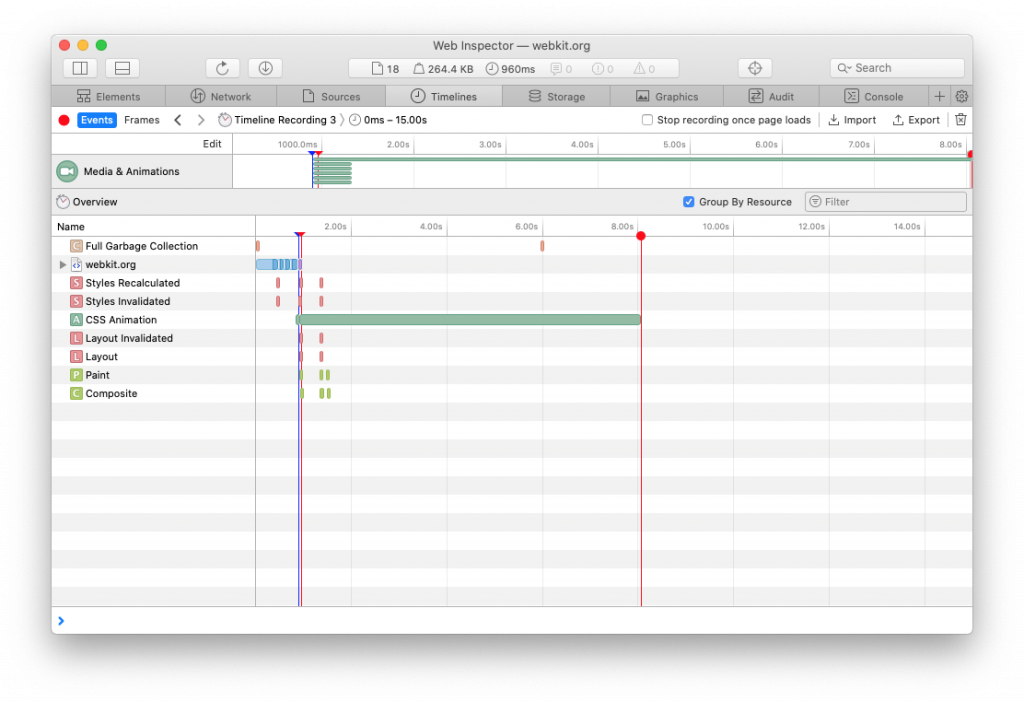
\includegraphics[width=.9\linewidth]{gorseller/safari13-web-animations.png}
\end{center}

Safari'nin bu sürümüyle birlikte eklenen bu API sayesinde artık CSS
animasyonlarını JavaScript tarafından yönetebileceğiz. Ayrıca tarayıcının Web
Inspector aracına animasyonları gösterebilecek "Media \& Animations" kısmı da
eklenmiş.
\subsection{\href{https://w3c.github.io/clipboard-apis/\#async-clipboard-api}{Async Clipboard API}}
\label{sec:org865f255}
W3C tarafından yeni bir web standardı olarak tanımlanan bu yeni API sayesinde
artık kullanıcıların clipboard'larına asenkron olarak erişip, kopyaladıkları
metinleri web sayfamız içerisinde amacımıza uygun olarak kullanabileceğiz.
Asenkron olmasının avantajı bu işlemler gerçekleştirilirken web sayfamız
tıkanmayacak. Aynı zamanda bu yeni API ile birden fazla farkı türden içeriği
kullanıcının panosuna gönderebilecek ve programlamasal olarak "Yapıştır"
işlemi yapabileceğiz. Mesela bu sayede artık kullanıcının panosunda "http"
ile bağlayan bir ifade varsa bunu \texttt{txtSiteUrl} metin kutusuna "Yapıştır" gibi
işlemleri yapabileceğiz.
\subsection{Sources Sekmesi}
\label{sec:org73d533f}
\begin{center}
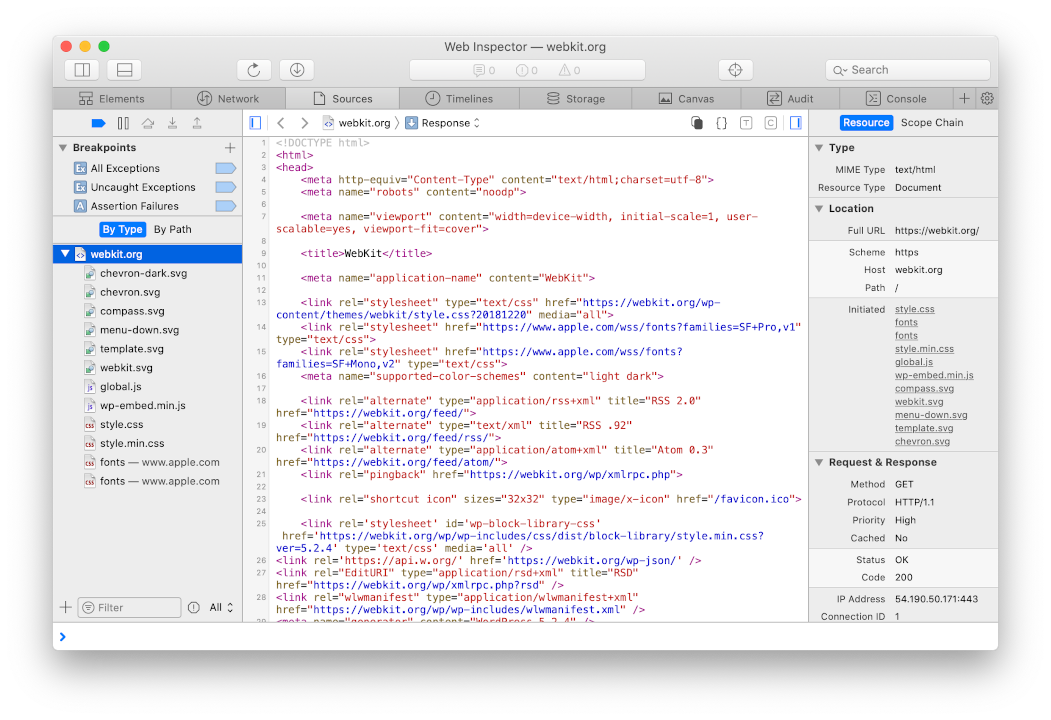
\includegraphics[height=6cm]{gorseller/safari13-sources-tab.png}
\end{center}

Tarayıcının Web Inspector aracına yeni eklenen bu sekme aslında önceki
Resources ve Debugger sekmelerinin birleştirilmiş ve iyileştirilmiş hali.
Üstelik artık yeni \href{https://webkit.org/web-inspector/javascript-breakpoints/}{JavaScript Breakpoint}'leri ile debug yapma özelliğine de
sahip.

Safari 13.1 sürümüyle gelen ve biz geliştiricileri ilgilendiren diğer özellik
ve değişiklikler için mutlaka konu başlığına eklediğim bağlantıya tıklayarak,
ilgi sayfayı incelemeyi unutmayın.
\section{StackOverflow'a \href{https://stackoverflow.blog/2020/03/30/introducing-dark-mode-for-stack-overflow/}{karanlık mod özelliği beta olarak geldi}}
\label{sec:org8d43dcd}
\begin{center}
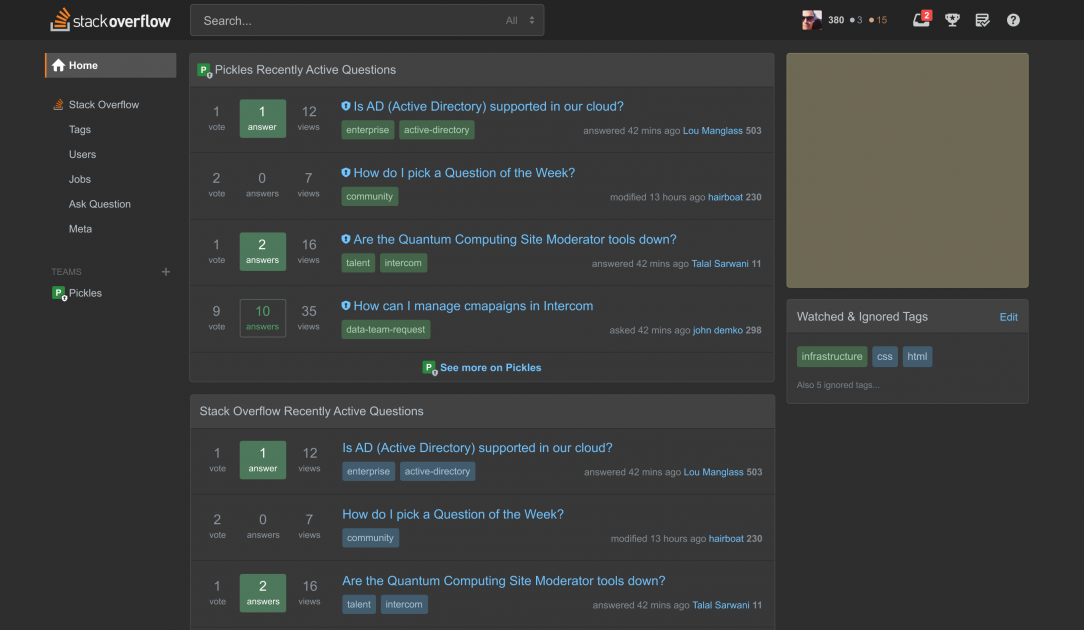
\includegraphics[width=.9\linewidth]{gorseller/stackoverflow-dark-mode.png}
\end{center}

Başlığı okuyunca ben de sizin gibi "Şimdiye kadar nasıl olmaz bu?!" dedim ama
yokmuş ve bu hafta eklenmiş. Aslında çeşitli eklentiler ile zaten biz karanlık
mod yapabiliyorduk ama sitenin kendinden desteklemesi daha iyi oldu. Bugüne
kadar olmaması başlı başına saçmalık zaten. Neyse geç olsun, güç olmasın
diyelim.

Temayı aktifleştirmek için \href{https://stackoverflow.com/users/preferences/current}{User Preferences} sayfasını açın ve "Theme"
kısmından istediğiniz temayı seçin ve işte! Artık geceleri StackOverflow'a
girince far görmüş tavşan gibi bakmayacaksınız ekrana :)
\section{\href{https://cs.opensource.google/}{Google açık kaynak projeleri için kod arama} sayfasını \href{https://opensource.googleblog.com/2020/04/code-search-for-google-open-source.html?m=1}{açtı}}
\label{sec:org936100f}
\begin{center}
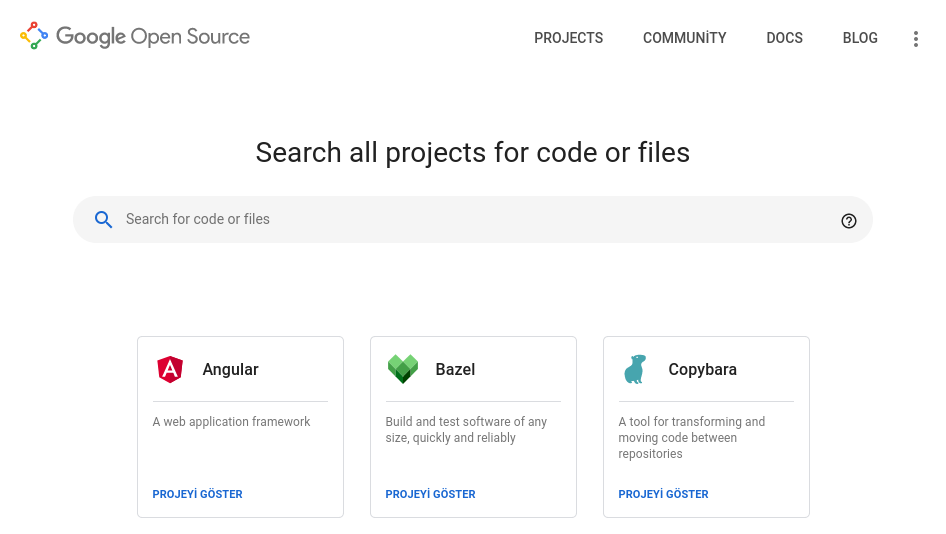
\includegraphics[width=.9\linewidth]{gorseller/google-code-search.png}
\end{center}

Google açık kaynak takımının bu hafta blogunda yayınladığı yazı ile artık
Google'ın tüm açık kaynak projelerinde arama yapabileceğimiz Code Search
sayfası kullanıma açıldı. Bu adresten sayfayı açarak siz de Google'ın açık
kaynak projeleri üzerinde dosya ya da kod araması yapabilirsiniz:
\url{https://cs.opensource.google/}

Aynı zamanda Android açık kaynak projesi için de bu sayfayı ziyaret
edebilirsiniz: \url{https://cs.android.com/}
\section{Diğer Haberler}
\label{sec:orgc812277}
\begin{itemize}
\item Microsoft, Koronavirüs yüzünden artan Azure kullanımlarıyla \href{https://mspoweruser.com/azure-overwhelmed-775-percent-demand-in-lockdown/}{başa çıkmaya
çalışıyor}.
\item Google, Chroma'daki SameSite Cookie değişikliklerini \href{https://blog.chromium.org/2020/04/temporarily-rolling-back-samesite.html?m=1}{geçici olarak geri
aldı}.
\item Google servis yönetimini kolaylaştıracak yeni \href{https://cloud.google.com/blog/products/networking/introducing-service-directory}{hizmetini beta olarak duyurdu}:
\href{https://cloud.google.com/service-directory}{Service Directory}.
\item Unreal Engine Wiki \href{https://forums.unrealengine.com/unreal-engine/announcements-and-releases/1739154-changes-to-the-official-unreal-engine-wiki}{kapatıldı}. Tüm wiki arşivi \href{https://epicgames.ent.box.com/s/2e5hhlvqyu9octooxbkgwt2xdmmrea9z}{buradan} indirilebiliyor.
\item Go dili için mikroservis framework'ü olan Go Micro, \href{https://github.com/micro/go-micro/releases/tag/v2.4.0}{v2.4.0 sürümünü
yayınladı}.
\item Nim programlama dilinin \href{https://nim-lang.org/blog/2020/04/03/version-120-released.html}{1.2.0 sürümü yayınlandı}.
\item Idris 2 programlama dilinin \href{https://www.idris-lang.org/idris-2-version-010-released.html}{0.1.0 sürümü yayınlandı}.
\item Rust programlama dilinin dokümantasyon \href{https://blog.rust-lang.org/inside-rust/2020/03/27/goodbye-docs-team.html}{takımı kapatıldı}.
\item Kotlin için GraphQL kütüphanesi graphql-kotlin, \href{https://github.com/ExpediaGroup/graphql-kotlin/releases}{2.0.0 sürümünü yayınladı}.
\item VueJS kütüphanesinin \href{https://github.com/vuejs/vue-next/releases/tag/v3.0.0-alpha.11}{v3.0.0-alpha.11 sürümü yayınlandı}.
\item Android için HTTP inspector aracı Chucker, \href{https://github.com/ChuckerTeam/chucker/releases/tag/3.2.0}{v3.2.0 sürümünü yayınladı}.
\item Sourcetrail aracının \href{https://www.sourcetrail.com/blog/release\_2020\_1/}{2020.1 sürümü yayınlandı}.
\item MultiCore OCaml projesi için \href{https://discuss.ocaml.org/t/multicore-ocaml-march-2020-update/5406}{Mart 2020 raporu} yayınlandı.
\item Sidekick Load Balancer \href{https://blog.min.io/introducing-sidekick-a-high-performance-load-balancer/}{aracı tanıtıldı}.
\item Prisma 2.0 Beta programı \href{https://www.prisma.io/blog/prisma-2-beta-b7bcl0gd8d8e}{duyuruldu}.
\item RapidFuzz kütüphanesinin \href{https://github.com/rhasspy/rapidfuzz/releases/tag/0.6.3}{0.6.3 sürümü çıktı}.
\item simdjson kütüphanesinin 0.3 sürümü \href{https://lemire.me/blog/2020/03/31/we-released-simdjson-0-3-the-fastest-json-parser-in-the-world-is-even-better/}{yayınlandı}.
\item Kubie aracı \href{https://blog.sbstp.ca/introducing-kubie/}{tanıtıldı}. \href{https://github.com/sbstp/kubie}{GitHub Deposu}
\item Eclipse Dirigible \href{https://www.dirigible.io/release/2020/04/04/news\_new\_release\_4\_4.html}{4.4 sürümü yayınlandı}.
\item Cortex \href{https://grafana.com/blog/2020/04/02/cortex-v1.0-released-the-highly-scalable-fast-prometheus-implementation-is-generally-available-for-production-use/}{v1.0 sürümü yayınlandı}.
\item dapr \href{https://github.com/dapr/dapr/releases/tag/v0.6.0}{v0.6.0 çıktı}.
\item libgit2 \href{https://github.com/libgit2/libgit2/releases/tag/v1.0.0}{v1.0.0 çıktı}.
\item sctructure \href{https://github.com/talyssonoc/structure/releases/tag/v2.0.0}{v2.0.0 çıktı}.
\item SpaceVim \href{https://spacevim.org/SpaceVim-release-v1.4.0/}{v1.4.0 çıktı}.
\end{itemize}
\section{Lisans}
\label{sec:orgdafaa76}
\begin{center}
\begin{center}

\includegraphics[height=1.5cm]{../../../img/CC_BY-NC-SA_4.0.png}
\end{center}

\href{yazilim-gundemi-2020-13.pdf}{Yazılım Gündemi - 2020/13} yazısı \href{https://erenhatirnaz.github.io}{Eren Hatırnaz} tarafından \href{http://creativecommons.org/licenses/by-nc-sa/4.0/}{Creative Commons
Atıf-GayriTicari-AynıLisanslaPaylaş 4.0 Uluslararası Lisansı} (CC BY-NC-SA 4.0)
ile lisanslanmıştır.
\end{center}
\end{document}
